\documentclass[a4paper,11pt]{article}
%\documentclass[a4paper,12]{article}
\pagestyle{empty}
\usepackage{amssymb}
\usepackage{amsmath}
\usepackage{graphicx}
\usepackage{epstopdf}
\usepackage{color}
\usepackage{hyperref}
% \usepackage[left=1.0in,top=1.0in,right=1.0in,bottom=2.5in]{geometry}
% \setlength{\textwidth}{6.75in}
% \setlength\topmargin{0.0in}
% \setlength\headheight{0.5in}
%\setlength{\topmargin}{0.25in}
%\setlength\headheight{0.25in}

\pdfpagewidth 8.5in
\pdfpageheight 11in 

\setlength\topmargin{0.25in}
\setlength\headheight{0.25in}
\setlength\headsep{0in}
\setlength\textheight{9in}
\setlength\textwidth{6.5in}
\setlength\oddsidemargin{0in}
\setlength\evensidemargin{0in}
\setlength\parindent{0.1in}
\setlength\parskip{0.25em}


\usepackage{fancyhdr,lastpage}
\pagestyle{fancy}
\chead{Supporting Effective Data~\thepage~of \pageref{LastPage}}
\fancyhead[L]{}
\fancyhead[R]{}
\cfoot{Page \thepage~of \pageref{LastPage}}

\newif\ifdraft
\drafttrue

\ifdraft
\newcommand{\fixme}[1]{ { \bf{ ***FIXME: #1 }} }
\newcommand{\jhanote}[1]{ {\textcolor{red} { ***Jha: #1 }}}
\else
\newcommand{\jhanote}[1]{}
\newcommand{\fixme}[1]{}
\fi

\begin{document}

%%%%% TITLE %%%%%
\begin{center}
\textbf {\large \bf Supporting Effective Data Placement on Heterogenous Distributed Platforms}
%\doublespacing

%%%%% AUTHORS %%%%%
\textbf {\normalsize \hspace{0.6 in} Miklos Erdelyim$^1$, Saurabh Sehgal$^2$, Andre Merzky$^3$,  \newline Katerina Stamou$^4$, Shantenu Jha$^{34*}$ }

%%%%% AFFILIATIONS %%%%%
\normalsize { \hspace{0.6 in} $^1$Department of Computer Science, \newline University of Pannonia, Veszprem, Hungary}

\normalsize { \hspace{0.6 in} $^2$ Edward S. Rogers Sr. Department of Electrical and Computer Engineering \newline University of Toronto}

\normalsize { \hspace{0.6 in} $^3$Center for Computation and Technology, \newline Louisiana State University, Baton Rouge, LA 70803, USA}

\normalsize {\hspace{0.6 in} $^4$Computer Science Department, \newline Louisiana State University, Baton Rouge, LA 70803, USA}

%\vspace{0.2in}
{\footnotesize {\hspace{0.0 in} $^*$Corresponding Author sjha@cct.lsu.edu}}

%\vspace{12pt}
\end{center}

%%%%% MAIN TEXT %%%%%

\vspace{12pt}

There are numerous scientific applications that utilize data and resources distributed over vast heterogeneous infrastructures and networks with varying speeds and characteristics. However, despite the drastic differences in hardware capabilities of such distributed systems, applications usually tend to utilize a single infrastructure for all of their computational and data processing needs. Since most distributed frameworks are designed with specific assumptions and infrastructures in mind, dependence on a single technology in a heterogeneous environment is not always an optimal choice to gain maximum runtime performance. For example, the Sector/Sphere data cloud is exclusively designed to support data-intensive computing on high speed networks, while other distributed filesystems like GFS/Hadoop assume limited bandwidth among infrastructure nodes [1]. Thus, for applications to efficiently utilize heterogeneous environments, abstractions must be developed for the efficient utilization of and orchestration across such distinct distributed infrastructure.  SAGA or “Simple API for Grid Applications” is a high level API that provides a simple, standard and uniform interface to the most commonly required distributed functionality [2]. SAGA can be used to encode grid applications, tool-kits to manage distributed applications as well as implement abstractions that support commonly occurring programming, access and usage patterns. Popular programming abstractions such as Map-Reduce and All-Pairs have been successfully implemented with SAGA to showcase its utilization as a flexible framework to scale-out data-intensive computations on different flavours of grids and clouds, and attain a high level of interoperability at the application level. Thanks to the ease of developing SAGA “Adaptors”, developers can provide SAGA the interfaces to interact with widely different infrastructures simultaneously throughout the execution of a single application.

This paper reports on progress on three-fronts: First, we take the existing SAGA Map-Reduce implementation, and enhance it to increase performance through adding features such as \fixme{Miklos insert things here} Secondly, we develop a SAGA adaptor for the Sector/Sphere compute and data cloud. The adaptor translates the high level SAGA job submission and file manipulation APIs into Sector/Sphere operations. This allows SAGA applications to leverage the functionality provided by the Sector/Sphere cloud for processing large data sets on infrastructures with high speed networks.  The third is the creation of components that facilitate flexibility in data placement relative to the computational resource -- that is either data can be transferred intelligently to match computational workloads or computational workloads can be placed to match (prevent) data requirements. More generically, it is worth mentioning that these approaches can be extend to support certain kinds of {\it affinities}.  

{\it Enhancing SAGA-based Map-Reduce Performance:} To orchestrate the functioning of the various different frameworks, we use the master-worker programming pattern, on which the SAGA Map-Reduce implementation is also based. This pattern allows the workers to execute on the different infrastructures (including Sector/Sphere) while communicating their progress and results through an advert DB to the master~\cite{sector}. \fixme{Miklos, please add}.

{\it Sector/Sphere Adaptors: }Sphere represents a programming paradigm that is different from MapReduce, and allows for a more general and wider approach to performing data intensive computations. Instead of using the more specific map/reduce implementations, an application can define any arbitrary functions to operate on data stored in the Sector cloud at multiple levels[1]. The Sector/Sphere adaptor drives the translation of the SAGA job submission APIs into executing the User Defined Functions or UDFs through Sphere on the Sector data cloud.  Specifically, the Sector/Sphere adaptor in conjunction with others (KFS, HDFS, Amazon EC2) naturally give us the opportunity to experiment with various distinct frameworks running on infrastructures best suited for their purposes. The SAGA MapReduce implementation utilizes these adaptors to submit jobs to the underlying heterogeneous infrastructure. With the enhancements to the SAGA Map-Reduce implementation combined with the Sector/Sphere adaptor, we describe in this paper, our approach to introduce intelligence in relative data-compute placement whilst demonstrating and utilizing the interoperability features inherent in the design of SAGA. 

{\it Validation Using Montage: } We test initial prototypes of these developments and their performance advantage using the well known Montage application.  Montage requires the execution of DAG;
% We introduce a SAGA application, digedag [Ref?], a part of the Montage project, already well under development. 
Digedag is a SAGA-based workflow planner and execution package, that provides APIs for translating abstract workflows in the form of DAGs into “concrete” DAGs, which are then executed on the underlying infrastructure.
% We use digedag as an example application running on a heterogeneous environment composed of various distributed frameworks and a large data distribution.
% Once a DAG has been translated into its concrete form,
We describe our approach to most efficiently execute it by taking into consideration the data-locality, as well as the access patterns of the execution steps required to complete the work flow. This analysis is done through developing performance models of transferring data between frameworks, as well as the distribution of the computing resources in the environment. Based on this analysis, the data is placed efficiently, and a subset of nodes and frameworks maybe chosen to perform the necessary computations. The shuffled data is also cached for future computations.



%%%%% REFERENCES %%%%%

\begin{thebibliography}{99}
\bibitem{sector} 
\newblock Y. Gu, R.L. Grossman, “Sector and Sphere: The Design and Implementation of a high performance data cloud”, Theme Issue of the Philosophical Transactions of the Royal Society A: Crossing Boundaries: Computational Science, E-Science and Global E-Infrastructure, 28 June 2009 vol. 367 no. 1897 2429-2445.

\bibitem{saga_ccgrid09}
\newblock C. Miceli, M. Miceli, S. Jha, H. Kaiser, A. Merzky, “Programming Abstractions for Data Intensive Computing on Clouds and Grids” ccgrid, pp.478-483, 2009 9th IEEE/ACM International Symposium on Cluster Computing and the Grid, 2009

\bibitem{montage} 
\newblock Montage ??

\bibitem{digedag} 
\newblock Developing Distributed Applications: A Case-Study of SAGA based Montage
to be submitted, IEEE e-Science Conference 2009 (Oxford)


\bibitem{Montage}
The Montage project, \url{http://montage.ipac.caltech.edu/}.

\bibitem{montagecloud}
E.~Deelman, G.~Singh, M.~Livny, B.~Berriman, and J.~Good, ``The cost of doing
 science on the cloud: the montage example,'' in \emph{SC '08: Proceedings of
  the 2008 ACM/IEEE conference on Supercomputing}.\hskip 1em plus 0.5em minus
  0.4em\relax Piscataway, NJ, USA: IEEE Press, 2008, pp. 1--12.


\end{thebibliography}

\vspace{12pt}

%%%%% FIGURES %%%%%

%================================================================
%  Add new figure (Figure 1) here
%================================================================
%\begin{figure}
%\centering
%\includegraphics[width=5.0in]{Image1.eps}
%\caption{CFD/MD Coupled Simulation on Channel Flow - Now Yet Included}
%\end{figure}
%================================================================

% \begin{figure}
% \centering
%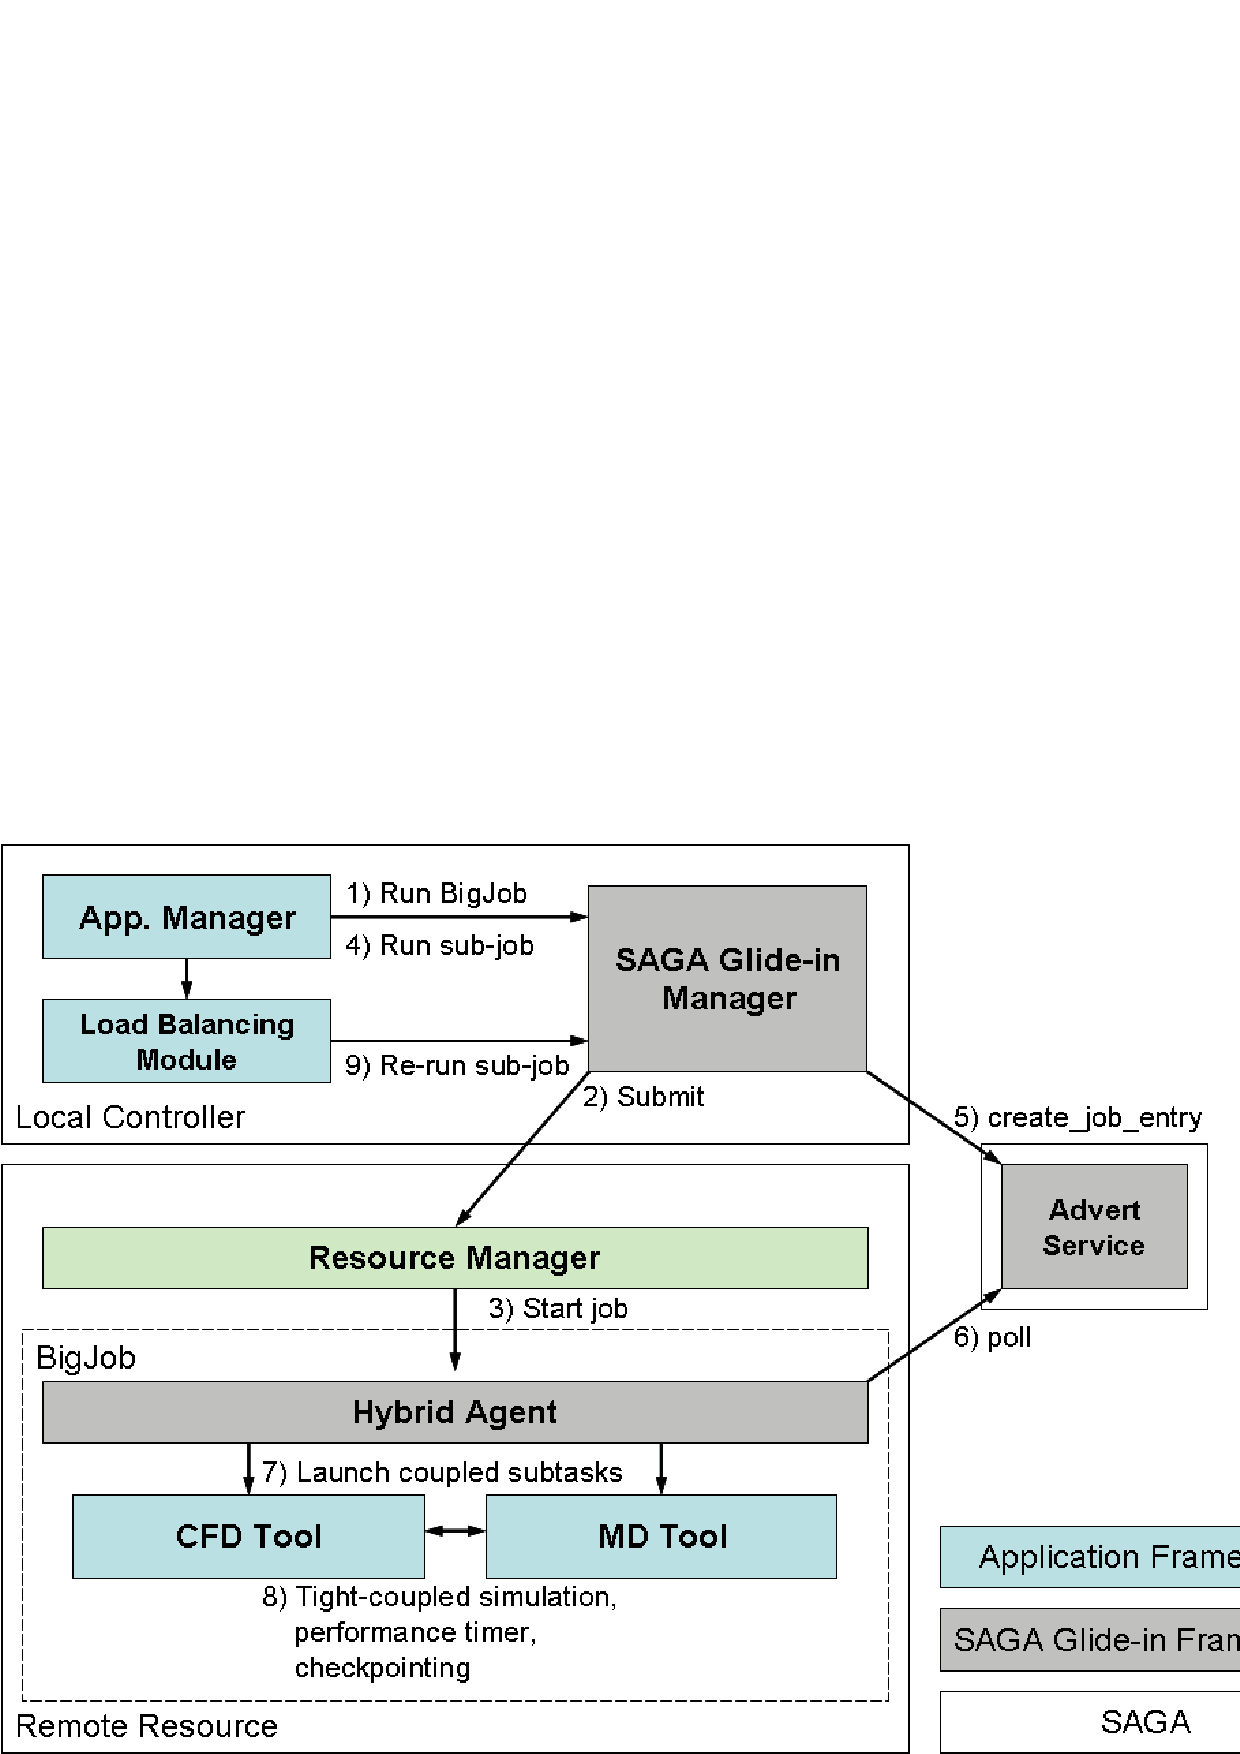
\includegraphics  [scale=0.33, angle=270]{Image2}
% \caption{Will I be a figure? \jhanote{}}
% \end{figure}

% \begin{figure}
% \centering
% %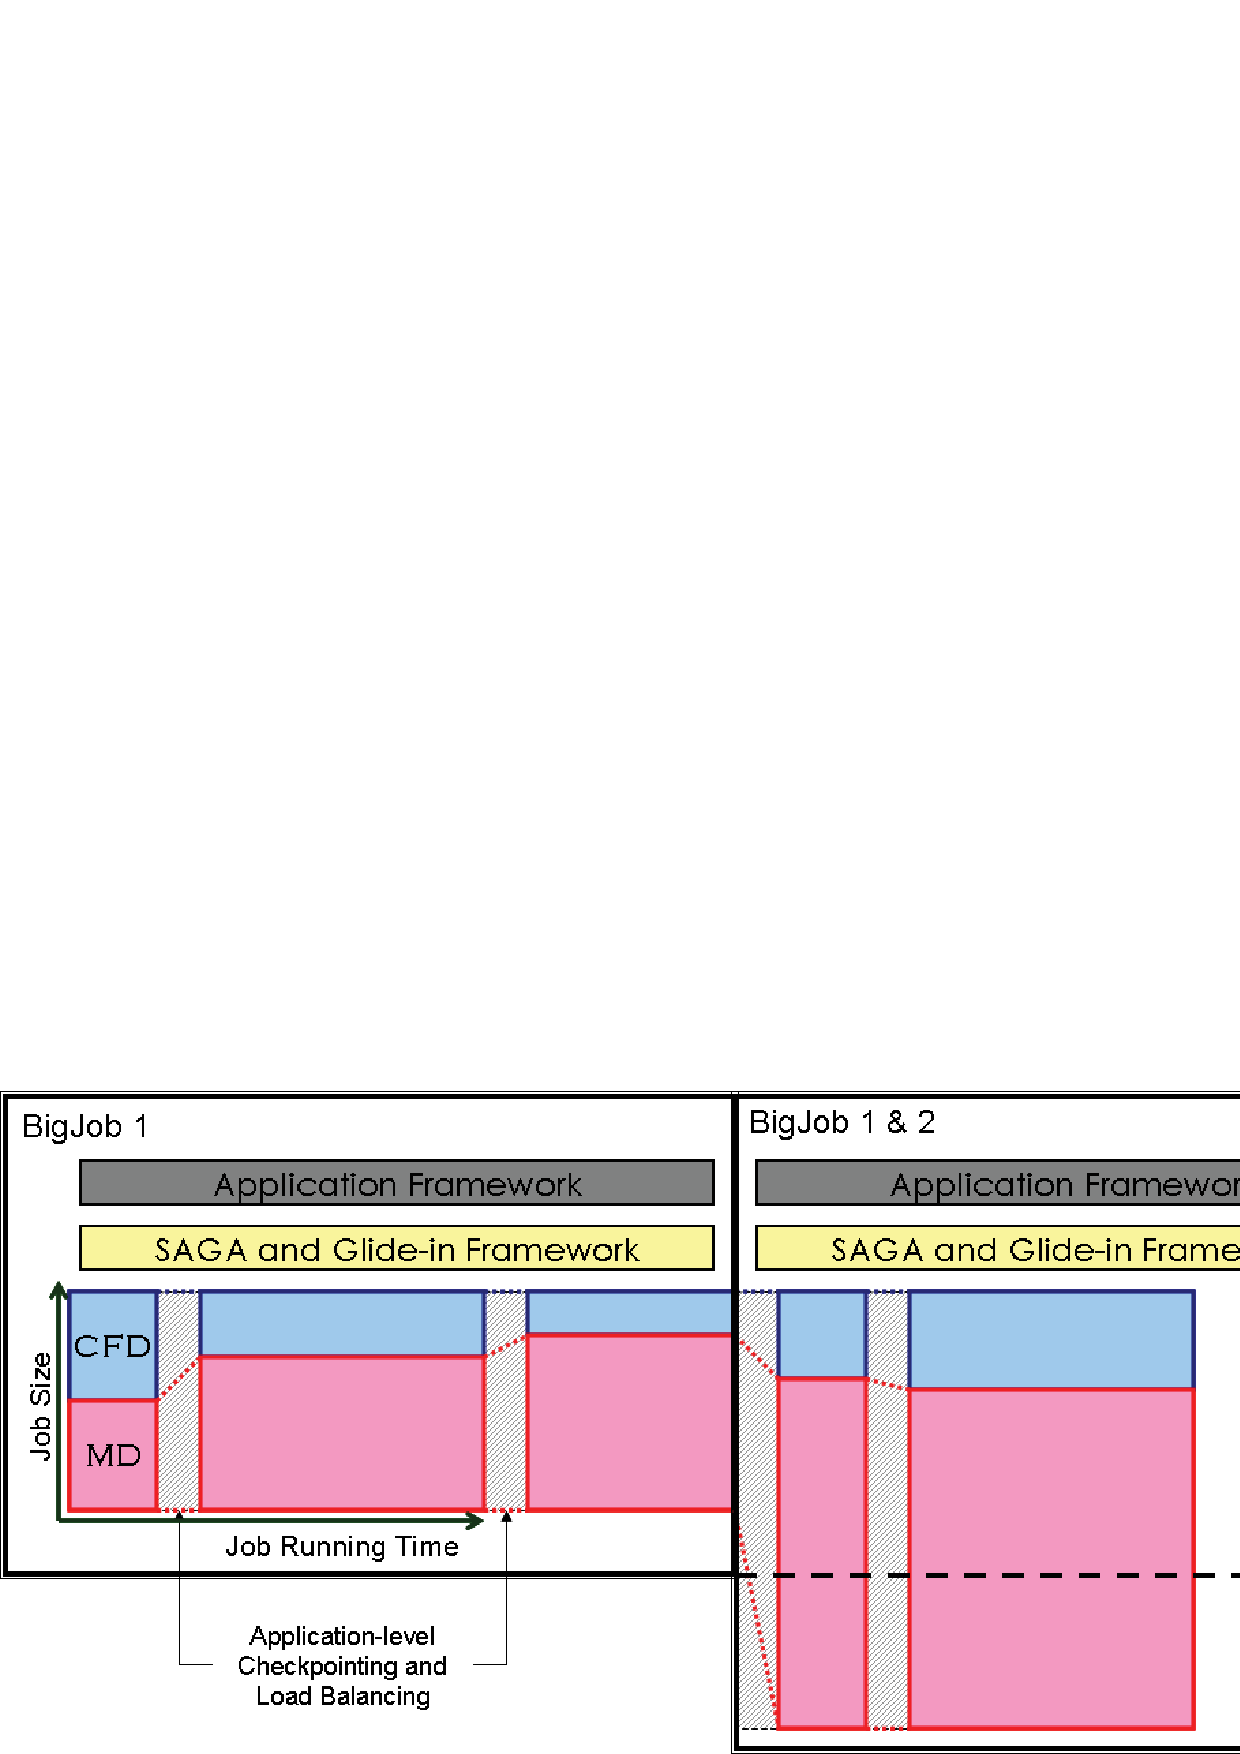
\includegraphics [scale=0.33, angle=270]{Image3}
% \caption{Will I be a figure? \jhanote{}}
% \end{figure}

\end{document}
